%; whizzy chapter
% -initex iniptex -latex platex -format platex -bibtex jbibtex -fmt fmt
% 以上 whizzytex を使用する場合の設定。

%     Kansai Debian Meeting resources
%     Copyright (C) 2007 Takaya Yamashita
%     Thank you for Tokyo Debian Meeting resources

%     This program is free software; you can redistribute it and/or modify
%     it under the terms of the GNU General Public License as published by
%     the Free Software Foundation; either version 2 of the License, or
%     (at your option) any later version.

%     This program is distributed in the hope that it will be useful,
%     but WITHOUT ANY WARRANTY; without even the implied warranty of
%     MERCHANTABILITY or FITNESS FOR A PARTICULAR PURPOSE.  See the
%     GNU General Public License for more details.

%     You should have received a copy of the GNU General Public License
%     along with this program; if not, write to the Free Software
%     Foundation, Inc., 51 Franklin St, Fifth Floor, Boston, MA  02110-1301 USA

%  preview (shell-command (concat "evince " (replace-regexp-in-string "tex$" "pdf"(buffer-file-name)) "&"))
% 画像ファイルを処理するためにはebbを利用してboundingboxを作成。
%(shell-command "cd image200708; ebb *.png")

%%ここからヘッダ開始。

\documentclass[mingoth,a4paper]{jsarticle}
\usepackage{kansaimonthlyreport}
\usepackage[dvips]{xy}


% 日付を定義する、毎月変わります。
\newcommand{\debmtgyear}{2008}
\newcommand{\debmtgdate}{14}
\newcommand{\debmtgmonth}{12}
\newcommand{\debmtgnumber}{20}

\begin{document}

\begin{titlepage}

% 毎月変更する部分、本文の末尾も修正することをわすれずに

 第\debmtgnumber{}回 関西 Debian 勉強会資料

\vspace{2cm}

\begin{center}
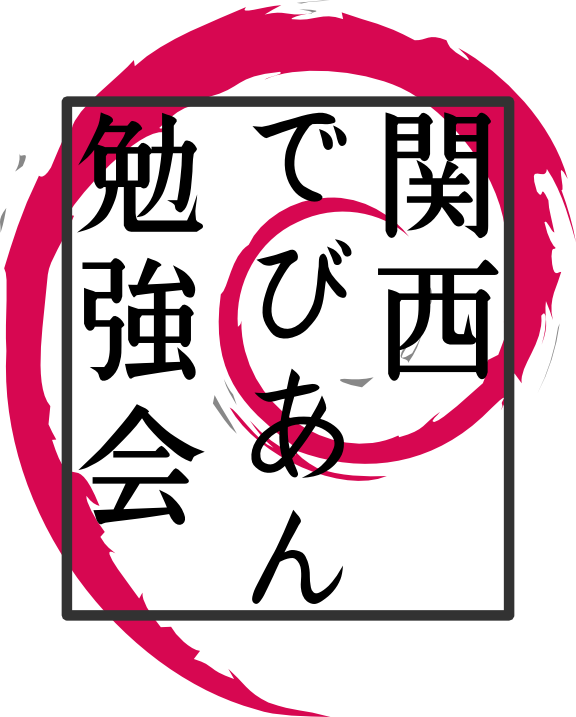
\includegraphics{image200802/kansaidebianlogo.png}
\end{center}

\begin{flushright}
\hfill{}関西 Debian 勉強会担当者 山下 尊也\\
\hfill{}\debmtgyear{}年\debmtgmonth{}月\debmtgdate{}日
\end{flushright}

\thispagestyle{empty}
\end{titlepage}

\dancersection{Introduction}{山下 尊也}
 
 関西 Debian 勉強会はDebian GNU/Linux のさまざ
 まなトピック(新しいパッケージ、Debian 特有の機能の仕組、Debian 界隈で起
 こった出来事、などなど)について話し合う会です。

 目的として次の三つを考えています。
 \begin{itemize}
  \item MLや掲示板ではなく、直接顔を合わせる事での情報交換の促進
  \item 定期的に集まれる場所
  \item 資料の作成
 \end{itemize}

 それでは、楽しい一時をお楽しみ下さい。

\newpage

\begin{minipage}[b]{0.2\hsize}
 {\rotatebox{90}{\fontsize{80}{80}
{\gt 関西デビアン勉強会}}}
\end{minipage}
\begin{minipage}[b]{0.8\hsize}
\hrule
\vspace{2mm}
\hrule
\setcounter{tocdepth}{1}
\tableofcontents
\vspace{2mm}
\hrule
\end{minipage}

\dancersection{KOF を終えて}{山下 尊也}

2008年11月7日(金)8日(土)に大阪南港ATCで開かれました 関西オープンソース
2008(以下、KOF) に
関西 Debian 勉強会は参加して来ました。

\subsubsection{セミナー企画、ステージ企画}

今回は、東京エリア Debian 勉強会からやまねさんに来て頂き、
セミナーとステージ企画を行なっていただきました。
当日の資料についてですが、\url{http://wiki.debian.org/HidekiYamane}にて
公開していますので、当日のセッションを見逃した方は、ご覧下さい。

\subsubsection{セミナー}

\begin{itemize}
 \item 『あなた』とオープンソース/フリーソフトウェア、そして『Debian』 やまねひでき
\end{itemize}

40人前後入る部屋でしたが、関係者を除いて35名入りほぼ満席でかなり盛況
だったと思います。

% また、担当者の手違いで土曜日ではなく金曜日のセミナーに
% なってしまいました。

\subsubsection{ステージ企画}

\begin{itemize}
 \item 2008/09 リリース予定 Debian 5.0 "Lenny" について やまねひでき
\end{itemize}

ステージ企画は、8日(土)に行なわれ16時5分から Ubuntu Japanese Team
の水野さんによる「Ubuntu 8.10ほかもろもろ」
が行なわれ、その後に16時35分からやまねさんのステージ企画だったため、
Ubuntu と一緒に話を聞く人が多かったです。

\subsubsection{配布物}

今回、配布しましたのは下記の2つになります。

\begin{itemize}
 \item Debian ``Lenny'' Live DVD
 \item 関西Debian勉強会、東京エリアDebian勉強会の情報が書かれたフライヤー
\end{itemize}

Debian ``Lenny'' Live DVDは、今月(2008年12月)の \TeX 講座
で使える状態に仕上げた Live DVD をのがたさんが中心になり、
作成しました。\footnote{詳しい情報は、
\url{http://wiki.debian.org/KansaiDebianMeetingKOF2008}を参考にして下さ
い。}
Debian Live の作成についての詳しい説明などは、来年やって頂けるそうです。

フライヤーは、オープンソースカンファレンス2008 Kansai(以下、OSC)
\footnote{\url{http://www.ospn.jp/osc2008-kansai/}}で配ったものとは、
違うものを配布しました。本来は、OSCと同様のものを配布したかったのですが、
DVD1枚の単価と、フライヤー1枚の単価を考えると
DVD1枚の単価の方が低かったため、実際にDebianに触って頂ける
DVDよりも高いフライヤーに対して意見が出たため、
今回は、A4サイズの紙を4分割し裁断し、A6サイズにしたものを
当日配布しました。

土曜日参加して頂いた Debian JP Projectのやまもとさんと
関西メンバーで話あった結果、1年単位で印刷した方がフライヤーの
コストを下げる事も出来るので、今後は、1年単位で東京と関西合同の
フライヤーを印刷したら良いかもって案も出ていました。

\subsubsection{物品販売}

\begin{itemize}
 \item Debian グッズ(Tシャツ、特製ステッカー)
 \item Debian 同人誌「あんどきゅめんてっどでびあん」 
\end{itemize}

物品販売は、OSCでも販売しましたステッカーとTシャツを
販売しました。
OSCで先にMサイズが売りきれてしまったため、今回は、
Lサイズのみの販売となりました。
また、2007年冬と2008年夏のコミックマーケットで販売された
「あんどきゅめんてっどでびあん」も販売しました。
「あんどきゅめんてっどでびあん」については、2008年冬号の
作成が終わっており、今月末に開かれるコミックマーケット75にて
販売される予定です。

売上については、\tbref{uriage}をご覧下さい。同人誌作成費用など
を抜いた金額を Debian JP Project に寄付する予定です。\footnote{2009年2月
下旬に行ないます。}

\begin{table}[htbp]
\caption{OSCでの売上}
\begin{center}
\begin{tabular}{|l|r|r|r|}
\hline
\multicolumn{1}{|c|}{} & \multicolumn{1}{c|}{単価} & \multicolumn{1}{c|}{個数} & \multicolumn{1}{c|}{合計} \\ \hline
あんどきゅめんてっど でびあん2008夏 & 1000 & 4 & 4000 \\ \hline
あんどきゅめんてっど でびあん2007冬 & 1000 & 5 & 5000 \\ \hline
あんどきゅめんてっど でびあん2007夏 & 1000 & 1 & 1000 \\ \hline
ステッカー(岩松) & 200 & 2 & 400 \\ \hline
ステッカー(のがた) & 100 & 1 & 100 \\ \hline
Tシャツ & 2000 & 2 & 4000 \\ \hline
合計 & \multicolumn{1}{l|}{} & \multicolumn{1}{l|}{} & 14500 \\ \hline
\end{tabular}
\end{center}
\label{uriage}
\end{table}

\dancersection{Debian 勉強会の資料を作成しよう}{山下 尊也}

\subsection{リポジトリのチェックアウト}

\begin{commandline}
$ git clone git://git.debian.org/git/tokyodebian/monthly-report
\end{commandline}

\begin{commandline}
$ make -j4 # エラーがでます
$ cp -p git-pre-commit.sh .git/hooks/pre-commit
$ make -j4
\end{commandline}

\subsection{emacs whizzytex の準備}

\begin{commandline}
$ cd XXXXX
$ emacs 
\end{commandline}

whizzytex\footnote{メンテナの上川さんによる資料が
\url{http://www.netfort.gr.jp/~dancer/column/whizzytex.html.ja}にありま
す。}を起動します。
プリビューが開始するというメリットだけでなく、即時コンパイルエラーを検出
できるのが重要です。

\begin{commandline}
M-x whizzytex-mode 
\end{commandline}

スペルチェックも起動しましょう。\footnote{iamerican もしくは ibritish パッ
ケージが必要です。}

\begin{commandline}
M-x flyspell-mode
\end{commandline}

\subsection{自分のセクションを追加する}
\label{sec:adddancersection}

まず自分のセクションを追加します。

\begin{commandline}
\dancersection{セクション名}{名前}
\index{XXXX@YYYY}
\label{XXXX@YYYY}

% 本文

\end{commandline}

\newpage

\subsection{セクションを追加}

\ref{sec:adddancersection}でセクションを追加しましたので、
次にサブセクションを追加していきます。必要があれば、サブサブセクションと
追加していきます。

\begin{commandline}

\subsection{xxxx} % サブセクション(小節)

\subsection{xxxx}

\subsubsection{xxxx} % サブサブセクション(少々節)

\end{commandline}

\subsection{注釈を追加する}

現時点で CDBS を使用しているソースパッケージは 1805 個、
ソースパッケージ全体の $\sim 16 \%$ だそうです
\footnote{これ、正しいですかね? }。

\begin{commandline}
現時点で CDBS を使用しているソースパッケージは 1805 個、
ソースパッケージ全体の $\sim 16 \%$ だそうです
\footnote{これ、正しいですかね? }。
\end{commandline}

\subsection{画像を追加する}
\label{sec:addpicture}

画像を追加する方法はいくつか方法がありますが、
eps ファイルだとファイルサイズが大きくなるため、
png や jpg などに変換を行なった上で追加した方が
良いと思います。

\begin{commandline}
M-! 
Shell command [~/monthly-report]$ cd image200808; ebb colinux_xlaunch_xdmcp.png
\end{commandline}

\begin{figure}[htbp]
 \begin{center}
  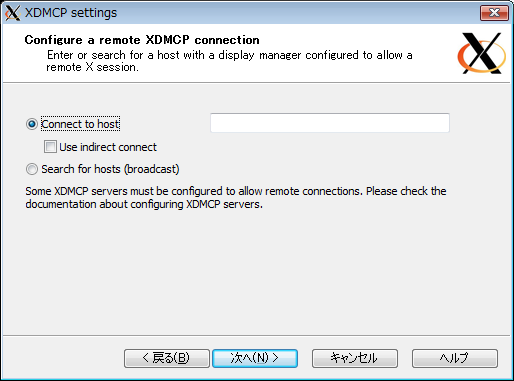
\includegraphics[width=100mm]{image200808/colinux_xlaunch_xdmcp.png}
 \end{center}
 \caption{XLaunch起動}
 \label{fig:colinux_xlaunch_xdmcp}
\end{figure}

\begin{commandline}
\subsection{画像を追加する}
\label{sec:addpicture}

\begin{figure}[htbp]
 \begin{center}
  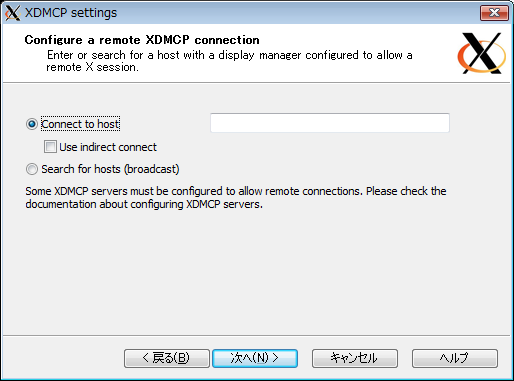
\includegraphics[width=100mm]{image200808/colinux_xlaunch_xdmcp.png}
 \end{center}
 \caption{XLaunch起動}
 \label{fig:olinux_xlaunch_xdmcp}
\end{figure}
\end{commandline}

\subsection{図や表を参照する}

monthlyreport では、図や表を参照するのに便利な
\verb|\fgrep{}|と\verb|\tbref{}|が
定義されています。

\ref{sec:addpicture}で紹介した\fgref{fig:colinux_xlaunch_xdmcp}

\begin{commandline}
\ref{sec:addpicture}で紹介した\fgref{fig:colinux_xlaunch_xdmcp}
\end{commandline}

\subsection{URL を追加してみる}

関西 Debian 勉強会の詳細については、\url{http://wiki.debian.org/KansaiDebianMeeting}にあります。

\begin{commandline}
関西 Debian 勉強会の詳細については、\url{http://wiki.debian.org/KansaiDebianMeeting}にあります。
\end{commandline}

\subsection{表を作ってみる}

\LaTeX で表を作る事も出来ますが、私は OpenOffice Calc で
表を作成し、\TeX のコードを生成してくれる
Calc2Latex\footnote{\url{http://calc2latex.sourceforge.net/indexj.html}}
を使っています。

\subsection{箇条書き}

来年度の予定は、
\begin{itemize}
 \item Live Helper のハンズオン
 \item 翻訳ハンズオン\\
\dots{}
\end{itemize}

Debian のインストールは、
\begin{enumerate}
 \item 言語設定
 \item キーボードの選択\\
\dots{}
\end{enumerate}

\begin{list}%
 {$\heartsuit$} %default label
 {Emacs が好きな理由} %formatting parameter
 \item カスタマイズ可能
 \item 指が覚えている
 \item Emacs の中だけでほとんどの作業が出来る\\
\dots{}
\end{list}

\begin{commandline}
\begin{itemize}
 \item Live Helper のハンズオン
 \item 翻訳ハンズオン\\
\dots{}
\end{itemize}

Debian のインストールは、
\begin{enumerate}
 \item 言語設定
 \item キーボードの選択\\
\dots{}
\end{enumerate}

\begin{list}%
 {$\heartsuit$} %default label
 {Emacs が好きな理由} %formatting parameter
 \item カスタマイズ可能
 \item 指が覚えている
 \item Emacs の中だけでほとんどの作業が出来る\\
\dots{}
\end{list}
\end{commandline}

\subsection{その他の注意事項}

\subsubsection{改行}

\LaTeX では、一般的な改行の解釈とは異なります。
空の行で段落の区切りと判断します。
段落として判断したら、行の頭に1文字分全角の空白が入ります。

\subsubsection{コマンドの結果について}

コマンドの結果などを簡単に載せられるように
kansaimonthlyreport.sty(元は、monthlyreport.sty) では、
commandline と言う勉強会用に定義されており、
commandline を利用した方が簡単です。

\subsubsection{エスケープが必要な文字列の出力方法}

\begin{itemize}
 \item \verb!\! verb は見にくくなるので最終的手段
 \item \~{}
 \item \^{}
 \item aaaa$<$aaaa そのままだと:<
 \item aaaa$>$aaaa そのままだと:>
 \item aaaa\#aaaa
 \item aaaa\%aaaa
 \item \_{}aaaa
\end{itemize}

\begin{itemize}
 \item {\tt /usr/share/iso-codes/iso\_3166.tab}
 \item /usr/share/iso-codes/iso\_{}3166.tab
\end{itemize}

\begin{commandline}
\begin{itemize}
 \item {\tt /usr/share/iso-codes/iso\_3166.tab}
 \item /usr/share/iso-codes/iso\_{}3166.tab
\end{itemize}
\end{commandline}

\subsubsection{全角英字などの禁止}

一般的に全角英字、半角カナの使用は使用しません。
これらの背景については、検索してみて下さい。

\dancersection{LaTeX beamer でプレゼンテーション}{大浦 真}

\subsection{はじめに}

\begin{itemize}
\item Debian勉強会などでは、講師をする際にプレゼン用の資料が必要になる。
\item どうやって作るか。
  \begin{itemize}
  \item MS Power Point や Openoffice.org の Impress。
  \item Magic Point。
  \item HTML とブラウザ。
  \item テキストファイルと less。
  \item \LaTeX{}で作る。
  \end{itemize}
\end{itemize}


\subsection{LaTeX beamer}

\subsubsection{特徴}

\begin{itemize}
\item \LaTeX{}がベース。
  \begin{itemize}
  \item 特別なことはしていないので、\LaTeX{}さえ分かれば使える。
  \end{itemize}
\item 最新版は 2007年3月リリースの 3.07。
\item 豊富なテーマ、豊富なサンプルが用意されている。
\item 簡単なアニメーションくらいはできる。
\item \verb|\section|、\verb|\subsection| を普通に使える。
\item 開発が盛ん。
  \begin{itemize}
  \item マニュアルは全 224ページ。
  \end{itemize}
\end{itemize}

\newpage

\subsubsection{インストール}


\begin{itemize}
\item \LaTeX{}一式が必要。Debian なら texlive をインストールする。
\item latex-beamer のインストール
  \begin{itemize}
  \item \url{http://latex-beamer.sourceforge.net/} からダウンロード。
  \item latex-beamer 以外にも pgf と xcolor も必要。
  \item Debian だったら、\texttt{\# apt-get install latex-beamer}
  \item 手動でインストールする場合は、
    \texttt{/usr/share/texmf} などに texmf という
    ディレクトリがあるので、
    texmf/tex/latex/beamer などのサブディレクトリを作って
    そこにスタイルファイルをコピー。
  \end{itemize}
\end{itemize}


\subsubsection{基本的な使い方}

\begin{itemize}
\item クラスファイルとして beamer.cls を使う。
  \begin{screen}
\begin{verbatim}
\documentclass{beamer}
\end{verbatim}
  \end{screen}
\item 使うテーマを決める。
  \begin{screen}
\begin{verbatim}
\usetheme{Boadilla}
\end{verbatim}
  \end{screen}
\item タイトル、作者、日付の設定。
  \begin{screen}
\begin{verbatim}
\title{LaTeX beamer でプレゼンテーション}
\author{大浦@Debian.org}
\date{2008年12月14日(日)}
\end{verbatim}
  \end{screen}
\item スライド一枚一枚はフレームと呼ばれる。
  フレームは\verb|\begin{frame}|と\verb|\end{frame}|で囲む。
\item タイトルページを作る。
  \begin{screen}
\begin{verbatim}
\begin{frame}
\titlepage{}
\end{frame}
\end{verbatim}
  \end{screen}
\item 必要なら目次のページを作る。
  \begin{itemize}
  \item 本文中で \verb|\section{}| などを使えば自動的に目次が作られる。
    テーマにもよるが、スライドの中にセクション名が表示される。
  \end{itemize}
  \begin{screen}
\begin{verbatim}
\begin{frame}
\frametitle{目次}
\tableofcontents{}
\end{frame}
\end{verbatim}
  \end{screen}
\item 適宜セクションに分ける。
\item プレゼンテーションは複数のフレームでできている。
\item \verb|\frametitle{}|がそのページのタイトル。
  \begin{screen}
\begin{verbatim}
\begin{frame}
\frametitle{はじめに}
\begin{itemize}
\item Debian勉強会などでは、講師をする際にプレゼン用の資料が必要になる。
  ....
\end{itemize}
\end{frame}
\end{verbatim}
  \end{screen}
\end{itemize}


\subsubsection{フレームとスライド}

\begin{itemize}
\item フレームは複数のスライドからできている。
\item \verb|\pause{}|を使うと一つのフレームを複数に分割できる。
  \begin{screen}
\begin{verbatim}
\begin{frame}
\frametitle{はじめに}
\begin{itemize}
\item Debian勉強会などでは、講師をする際にプレゼン用の資料が必要になる。
\pause{}
\item どうやって作るか。
    ....
\end{itemize}
\end{frame}
\end{verbatim}
  \end{screen}
\item 特定のスライドだけでコマンドを有効にできる。
\item \LaTeX{}のコマンドの後に \verb|< >| を付ける。
  \begin{screen}
\begin{verbatim}
\begin{itemize}
\item \textbf{この行は常に太字です。}
\item \textbf<2>{この行は2枚目のスライドでのみ太字です。}
\item \textbf<3>{この行は3枚目のスライドでのみ太字です。}
\end{itemize}
\end{verbatim}
  \end{screen}
\end{itemize}


\subsubsection{簡単なアニメーション}


\begin{itemize}
\item ごく簡単なアニメーションが使える。
\item \verb|\animate| と \verb|\animatevalue| を使う。
  \begin{screen}
\begin{verbatim}
\newcount\opaqueness
\begin{frame}
  ....
\animatevalue<1-10>{\opaqueness}{100}{0}
\begin{colormixin}
{\the\opaqueness!averagebackgroundcolor}
この文字列はフェードアウトします。
\end{colormixin}
\end{frame}
\end{verbatim}
  \end{screen}
\end{itemize}


\subsubsection{画像の取り込み}

\begin{itemize}
\item \LaTeX{}なので普通に画像も取り込める。
\item 例えば Debian の logo。\texttt{openlogo.eps}
\item \texttt{graphicx.sty} を使う。
  \begin{screen}
\begin{verbatim}
\includegraphics[height=3cm,keepaspectratio,clip]{openlogo.eps}
\end{verbatim}
  \end{screen}
\end{itemize}

\subsection{プレゼンの方法}

\begin{itemize}
\item dvi ファイルを作って、xdvi でプレビューすると画像が表示されないが、
  作成途中のプレビューには十分。
\item プレゼンの際には、Postscript か PDF に変換する。
\item Postscript にする場合は、dvips を使う。
  \begin{itemize}
  \item \texttt{beamer.cls}にオプション\texttt{dvips}を付ける。
    \verb|\documentclass[dvips]{beamer}|
  \item pspresent を使って表示。
    \url{http://www.cse.unsw.edu.au/~matthewc/pspresent/}
  \end{itemize}
\item PDF にする場合は、dvipdfmx か、
  Postscript に変換してから Ghostscript (ps2pdf) を使う。
  \begin{itemize}
  \item dvipdfmx を使うためには、\texttt{beamer.cls}に
    オプション\texttt{dvipdfm}を付ける。
  \item Acrobat Reader を使って表示。hyperlink の機能も使える。
  \end{itemize}
\item 配布用の資料ではアニメーションなどは無効にする。
  アニメーションは複数ページとして扱われるので、それを1ページにする。
  \begin{itemize}
  \item \texttt{beamer.cls}にオプション\texttt{handout}を付ける。
  \end{itemize}
\item Postscript から印刷する場合は、psutils に含まれる
  psnup で 1ページに複数のフレームを入れて印刷。
  \begin{itemize}
  \item psutils
    \url{http://www.dcs.ed.ac.uk/home/ajcd/psutils/}
  \end{itemize}
\end{itemize}


\subsubsection{終わりに}


\begin{itemize}
\item \LaTeX{}の使い方さえ分かっていれば
  latex-beamer は簡単に使えます。
\item \LaTeX{}上の他のプレゼンテーションスタイルよりも
  派手なスライドを作れます。
\item ぜひ、latex-beamer を使って Debian 勉強会で講師をしましょう。
\end{itemize}

\dancersection{来年の関西 Debian 勉強会について}{山下 尊也}

\subsection{過去のDebian勉強会を振り返って}

各種勉強会の過去の実施実績をまとめます。
東京エリアDebian勉強会と、関西Debian勉強会について整理します。
グラフにしてみると\fgref{fig:peoplechart}になります。
\begin{figure}[h]
 \begin{center}
  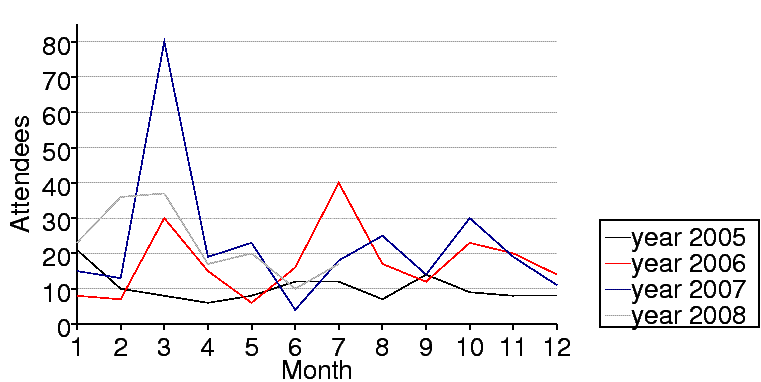
\includegraphics[width=0.45\hsize]{image200812/people-chart.png}
  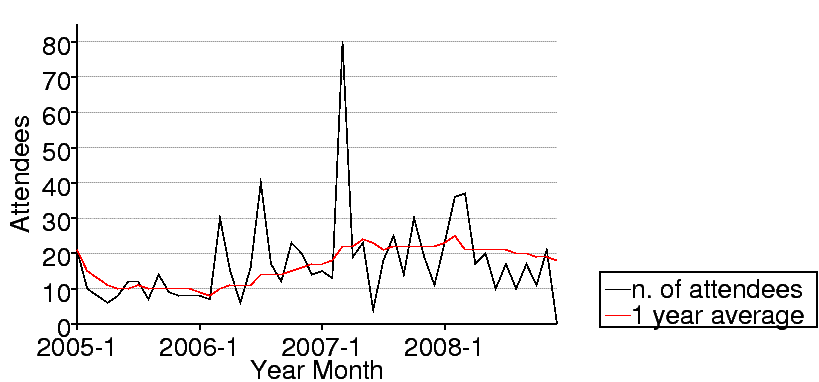
\includegraphics[width=0.45\hsize]{image200812/serialized.png}
 \end{center}
\caption{参加人数推移}
\label{fig:peoplechart}
\end{figure}

関西の状況を確認してみましょう。
\fgref{fig:kansaipeoplechart}になります。
毎月20名程度の参加者がいる事が分かると思います。

\begin{figure}[h]
 \begin{center}
  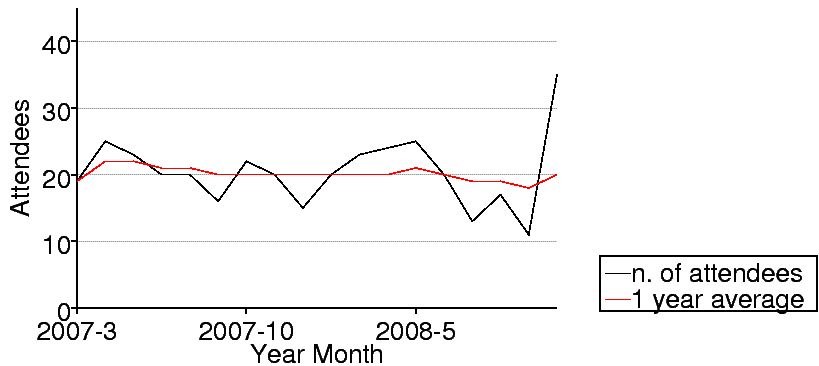
\includegraphics[width=0.45\hsize]{image200812/kansai.png}
 \end{center}
\caption{関西の参加人数推移}
\label{fig:kansaipeoplechart}
\end{figure}

表で見てみましょう。
 
 \begin{table}[ht]
\begin{minipage}{0.5\hsize}
 \caption{東京エリアDebian勉強会参加人数(2005年)}\label{tab:count}
 \begin{center}
  \begin{tabular}{|l|c|p{10em}|}
 \hline
   & 人数 & 内容 \\
 \hline
   2005年1月 & 21 & 秘密\\
   2005年2月 & 10 & debhelper1\\
   2005年3月 & 8 &  (早朝) debhelper2、social contract\\
   2005年4月 & 6 & debhelper3\\
   2005年5月 & 8 & DFSG、dpkg-cross、lintian/linda\\
   2005年6月 & 12 & alternatives、d-i\\
   2005年7月 & 12 & toolchain、dpatch\\
   2005年8月 & 7 & Debconf参加報告、ITPからアップロードまで\\
   2005年9月 & 14 & debconf\\
   2005年10月 & 9 & apt-listbugs、バグレポート、debconf翻訳、debbugs\\
   2005年11月 & 8 & DWN翻訳フロー、statoverride\\
   2005年12月 & 8 & 忘年会\\
 \hline
  \end{tabular}
 \end{center}
\end{minipage}
\begin{minipage}{0.5\hsize}
 \caption{東京エリアDebian勉強会参加人数(2006年)}\label{tab:count2006}
 \begin{center}
  \begin{tabular}{|l|c|p{10em}|}
 \hline
 & 参加人数 & 内容\\
 \hline
 2006年1月 & 8 & policy、Debian勉強会でやりたいこと\\
 2006年2月 & 7 & policy、multimedia \\
 2006年3月 & 30 & OSC: debian勉強会、sid \\
 2006年4月 & 15 & policy、latex \\
 2006年5月 & 6 & mexico \\
 2006年6月 & 16 & debconf、cowdancer\\
 2006年7月 & 40 & OSC-Do: MacBook Debian \\
 2006年8月 & 17 & 13執念 \\
 2006年9月 & 12 & 翻訳、Debian-specific、oprofile \\
 2006年10月 & 23 & network、i18n会議、Flash、apt \\
 2006年11月 & 20 & 関西開催: bug、sid、packaging \\
 2006年12月 & 14 & 忘年会 \\
 \hline
  \end{tabular}
 \end{center}
\end{minipage}
 \end{table}

\begin{table}[!b]
\begin{minipage}{0.5\hsize}
 \caption{東京エリアDebian勉強会参加人数(2007年)}\label{tab:count2007}
 \begin{center}
  \begin{tabular}{|l|c|p{10em}|}
 \hline
 & 参加人数 & 内容\\
 \hline
2007年1月 & 15 & 一年を企画する \\
2007年2月 & 13 & dbs, dpatch\\ 
2007年3月 & 80 & OSC仮想化 \\
2007年4月 & 19 & quilt, darcs, git\\
2007年5月 & 23 & etch, pbuilder, superh \\   
2007年6月 & 4 & エジンバラ開催:Debconf7 実況中継 \\
2007年7月 & 18 & Debconf7 参加報告\\
2007年8月 & 25 & cdn.debian.or.jp \\   
2007年9月 & 14 & exim \\   
2007年10月 & 30 & OSC Tokyo/Fall(CUPS) \\   
2007年11月 & 19 & live-helper, tomoyo linux kernel patch, server\\
2007年12月 & 11 & 忘年会\\
 \hline
  \end{tabular}
 \end{center}
\end{minipage}
\begin{minipage}{0.5\hsize}
 \caption{東京エリアDebian勉強会参加人数(2008年)}\label{tab:count2008}
 \begin{center}
  \begin{tabular}{|l|c|p{10em}|}
 \hline
 & 参加人数 & 内容\\
 \hline
2008年1月 & 23 & 一年を企画する \\
2008年2月29+1日 & 36 & OSC  \\
2008年3月 & 37 & データだけのパッケージ、ライセンス \\
2008年4月 & 17 & バイナリパッケージ \\
2008年5月 & 20 & 複数のバイナリパッケージ \\
2008年6月 & 10 & debhelper \\
2008年7月 & 17 & Linux kernel patch / module パッケージ \\
2008年8月 & 10 & Debconf IRC会議とDebian温泉 \\
2008年9月 & 17 & po4a, 「Debian メンテナのお仕事」 \\
2008年10月 & 11? & OSC Tokyo/Fall \\
2008年11月 & 17 & LaTeX 原稿作成合宿 \\
2008年12月 & ? & 忘年会 \\
 \hline
  \end{tabular}
 \end{center}
\end{minipage}
\end{table}

\begin{table}[!t]
\begin{minipage}{0.5\hsize}
 \caption{関西Debian勉強会参加人数(2007年)}\label{tab:count2007kansai}
 \begin{center}
  \begin{tabular}{|l|c|p{10em}|}
 \hline
 & 参加人数 & 内容 \\
 \hline
2007年3月 & 19 & 開催にあたり \\
2007年4月 & 25 & goodbye、youtube、プロジェクトトラッカー\\
2007年6月 & 23 & 社会契約、テーマ、debian/rules、bugreport\\
2007年7月 & 20前後 & OSC-Kansai \\
2007年8月 & 20 & Inkscape、patch、dpatch\\
2007年9月 & 16 & ライブラリ、翻訳、debtorrent\\
2007年10月 & 22& 日本語入力、SPAMフィルタ\\
2007年11月 & 20前後 & KOF \\   
2007年12月 & 15& 忘年会、iPod touch\\   
 \hline
  \end{tabular}
 \end{center}
\end{minipage}
\begin{minipage}{0.5\hsize}
 \caption{関西Debian勉強会参加人数(2008年)}\label{tab:count2008kansai}
 \begin{center}
  \begin{tabular}{|l|c|p{10em}|}
 \hline
 & 参加人数 & 内容 \\
 \hline
2008年2月 & 20 & PC Cluster, GIS, \TeX \\
2008年3月 & 23 & bug report, developer corner, GPG \\
2008年4月 & 24 & coLinux, Debian GNU/kFreeBSD, sid \\
2008年5月 & 25  & ipv6, emacs, ustream.tv\\
2008年6月 & 20  & pbuilder, hotplug, ssl\\
2008年8月 & 13  & coLinux \\
2008年9月 & 17  & debian mentors, ubiquity, DFSG\\
2008年10月 & 11  & cdbs,cdn.debian.or.jp \\
2008年11月 & 35  & KOF \\
2008年12月 & ?  & LaTeX,LaTeX beamer\\
 \hline
  \end{tabular}
 \end{center}
\end{minipage}
\end{table}

\newpage

\subsection{来年の関西Debian勉強会}

\subsubsection{イベント開催参加について}

来年のイベントについては、大幅な変更が無ければ、
昨年度と同様にOSC Kyotoは7月。KOFは11月頃に開かれると思います。
東京と共同でフライヤーを作る事になると来年の2,3月にOSC Tokyo Springが
開かれる予定ですので、これらを考慮に入れて、フライヤーを作らないといけま
せん。

\subsubsection{通常の勉強会}

みなさんは、どのような勉強会が良いですか?
次のページにメモがありますので、自分の開きたい開いてほしい勉強会を
書いてみて、ディスカッションを行い来年度の予定を決めましょう。

\newpage

\dancersection{メモ}{}
\mbox{}\newpage

\mbox{}\newpage

\printindex
 \cleartooddpage

 \begin{minipage}[b]{0.2\hsize}
  \rotatebox{90}{\fontsize{80}{80} {\gt 関西デビアン勉強会} }
 \end{minipage}
 \begin{minipage}[b]{0.8\hsize}

 \vspace*{15cm}
 \rule{\hsize}{1mm}
 \vspace{2mm}
 
\includegraphics[width=2cm]{image200502/openlogo-nd.eps}
 \noindent \Large \bf Debian 勉強会資料\\ \\
 \noindent \normalfont \debmtgyear{}年\debmtgmonth{}月\debmtgdate{}日 \hspace{5mm}  初版第1刷発行\\
 \noindent \normalfont 関西 Debian 勉強会 (編集・印刷・発行)\\
 \rule{\hsize}{1mm}
 \end{minipage}

\end{document}
